% vim: set spell spelllang=en tw=100 et sw=4 sts=4 :

\documentclass[a4paper]{article}

\usepackage[inner=1in,outer=1in,top=1in,bottom=1in]{geometry}
\usepackage{microtype}                 % the pretty
\usepackage{tikz}                      % For pretty pictures

\usetikzlibrary{arrows, shadows, calc, positioning, decorations, decorations.pathmorphing,
    decorations.pathreplacing, patterns, tikzmark, fit}

\begin{document}

\pagestyle{empty}

\begin{center}
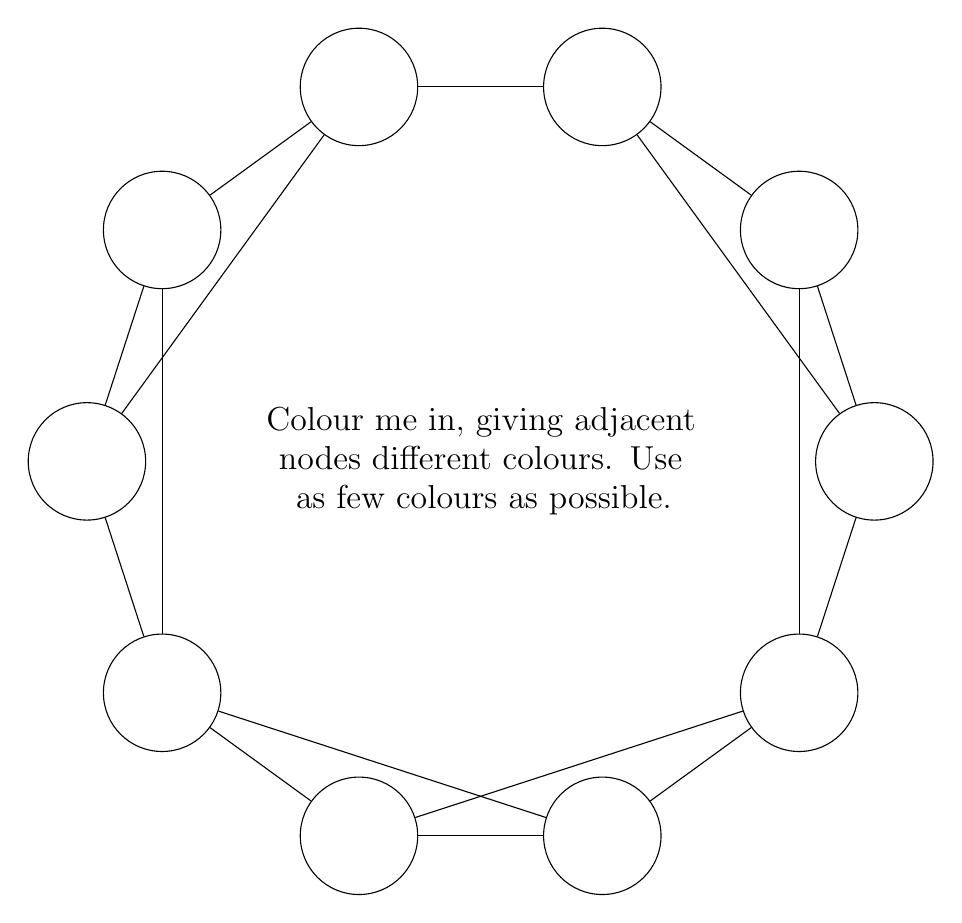
\begin{tikzpicture}

    \node [anchor=center, font=\large, text width=6cm, align=center]{
        Colour me in, giving adjacent nodes different colours. Use as few colours as possible. };

    \newcount \c
    \foreach \n in {0, ..., 9}{
        \c=\n
        \multiply\c by -36
        \advance\c by 90
        \advance\c by 18
        \node[draw, circle, inner sep=15pt, font=\large] (N\n) at (\the\c:5) {~};
    }

    \draw (N0) -- (N1);
    \draw (N1) -- (N2);
    \draw (N1) -- (N3);
    \draw (N2) -- (N3);
    \draw (N2) -- (N4);
    \draw (N3) -- (N4);
    \draw (N4) -- (N5);
    \draw (N4) -- (N6);
    \draw (N5) -- (N6);
    \draw (N5) -- (N7);
    \draw (N6) -- (N7);
    \draw (N7) -- (N8);
    \draw (N7) -- (N9);
    \draw (N8) -- (N0);
    \draw (N8) -- (N9);
    \draw (N9) -- (N0);

\end{tikzpicture}
\end{center}

\vspace{4em}

\begin{center}
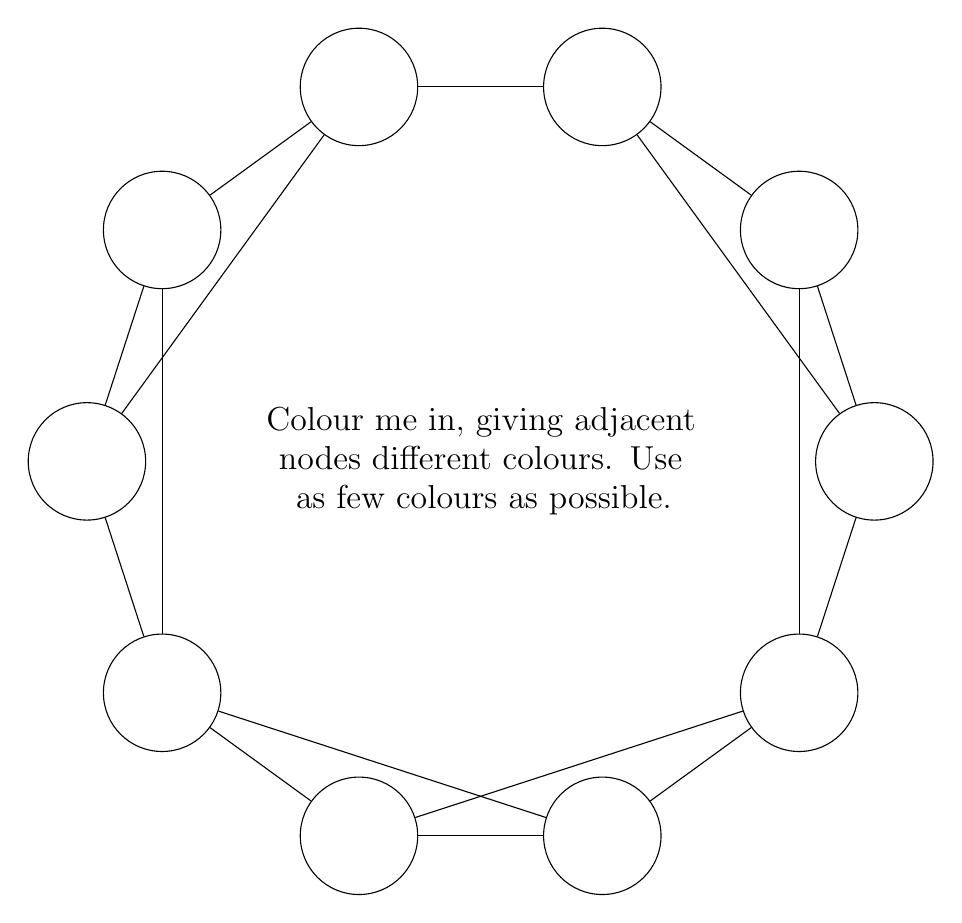
\begin{tikzpicture}

    \node [anchor=center, font=\large, text width=6cm, align=center]{
        Colour me in, giving adjacent nodes different colours. Use as few colours as possible. };

    \newcount \c
    \foreach \n in {0, ..., 9}{
        \c=\n
        \multiply\c by -36
        \advance\c by 90
        \advance\c by 18
        \node[draw, circle, inner sep=15pt, font=\large] (N\n) at (\the\c:5) {~};
    }

    \draw (N0) -- (N1);
    \draw (N1) -- (N2);
    \draw (N1) -- (N3);
    \draw (N2) -- (N3);
    \draw (N2) -- (N4);
    \draw (N3) -- (N4);
    \draw (N4) -- (N5);
    \draw (N4) -- (N6);
    \draw (N5) -- (N6);
    \draw (N5) -- (N7);
    \draw (N6) -- (N7);
    \draw (N7) -- (N8);
    \draw (N7) -- (N9);
    \draw (N8) -- (N0);
    \draw (N8) -- (N9);
    \draw (N9) -- (N0);

\end{tikzpicture}
\end{center}

\end{document}

